\chapter{Fundamentos}
\label{cha:fundamentos}
	
	Nesse capítulo é apresentada a revisão bibliográfica necessária para a fundamentação dos capítulos subsequentes.
	
	Seis conceitos básicos são apresentados: ``Indústria 4.0'', ``Logística \& Cadeia de Suprimentos'', ``Ciclo de vida do produto'', ``Memória digital do produto'', ``Arquitetura orientada a serviços'' e ``Modelagem de sistemas''.
	
	A inter-relação entre esses conceitos é a base para o entendimento e criação da arquitetura para o compartilhamento de informações sobre o ativo ao longo da cadeia de suprimentos e para a elaboração de considerações sobre implicações do massivo compartilhamento de informações no ciclo de vida do produto no contexto da Indústria 4.0.

\section{Indústria 4.0}
\label{sec:industria4}

	Indústria 4.0 (I4.0) é o nome dado às recentes modificações em relação às tecnologias utilizadas em processos industriais e à forma de organização dos sistemas industriais. Tais tecnologias são inseridas com o propósito de se oferecer um alto nível de automação e intercâmbio de informações entre equipamentos e produtos \cite{lasi2014industryfour}.

	O nome I4.0 se dá pelo fato de ser considerada a quarta grande revolução com relação às tecnologias de produção industrial, sendo as ``revoluções industriais'' consideradas evoluções tecnológicas que levaram a grandes mudanças no paradigma de produção. As outras transições dentro da indústria ao longo da história aconteceram: no campo da mecanização da produção (1\textsuperscript{a} revolução industrial), com a produção em massa e intenso uso de energia elétrica (2\textsuperscript{a} revolução industrial) e com a expansão da automação e eletrônica (3\textsuperscript{a} revolução industrial) \cite{lasi2014industryfour}. Tal histórico de revoluções no campo da indústria é ilustrado na \autoref{fig:i4-2}.

	\begin{figure}[htb]
		\centering
		\caption{Evolução da indústria por meio das revoluções industriais.}
		\label{fig:i4-2}
		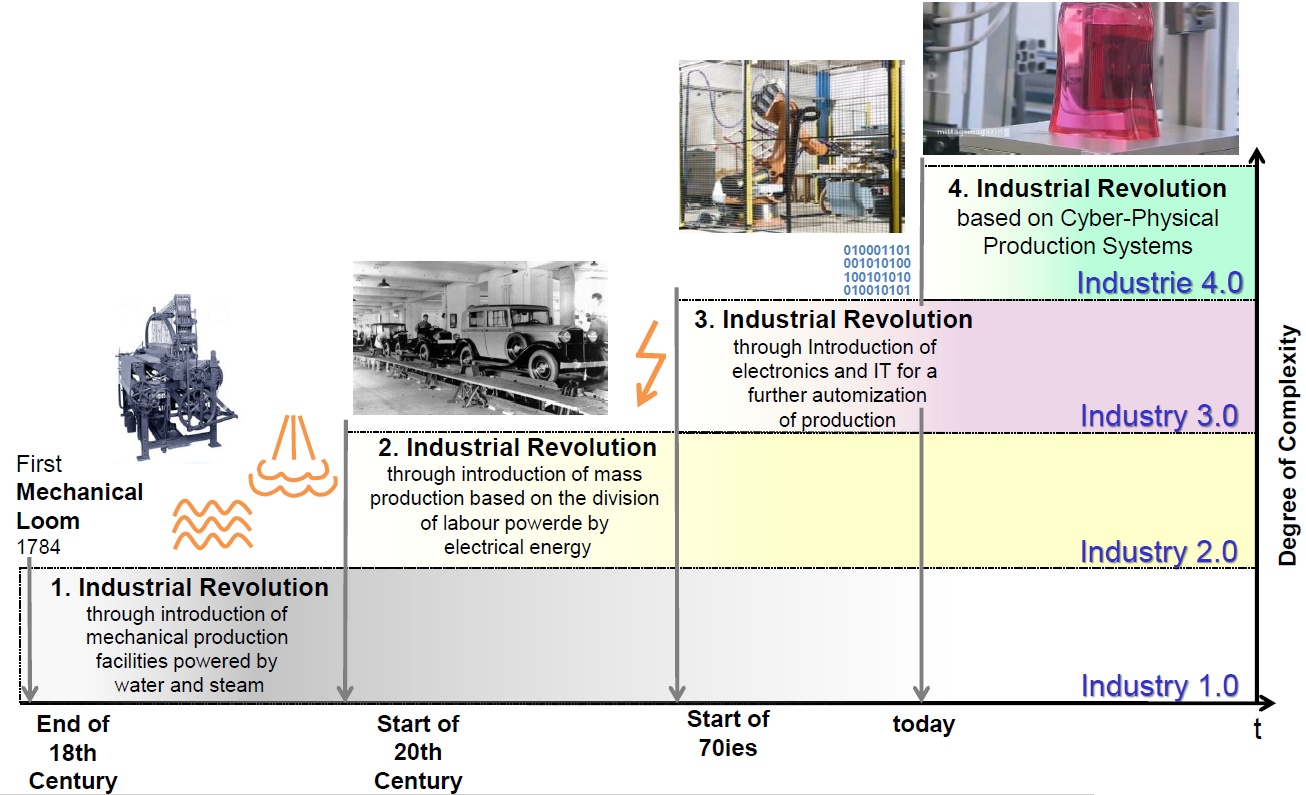
\includegraphics[width=1\textwidth]{i4-2.png}
		\fonte{\citeonline{wahlster2013industrie} (adaptado). }
	\end{figure}

	O termo I4.0 foi trazido a público pela primeira vez em 2011 na feira industrial de Hanôver (\textit{Hannover-Messe}) \cite{kagermann2011industrie}, que é uma feira tecnológica de grande relevância internacional e tem o costume de apresentar grandes inovações relacionadas ao setor industrial.

	Por vezes, a I4.0 é tratada também como a convergência da produção industrial com as novas Tecnologias de Informação e Comunicação (TIC) \cite{hermann2016design}.
	
	Embora o termo I4.0 seja bastante comum na discussão tecnológica atual, muitas empresas, centros de pesquisa e universidades não mantêm uma definição comum sobre o assunto. Segundo \citeonline{hermann2016design} e com base em uma revisão de literatura feita pelos mesmos autores, a I4.0 é composta por quatro princípios de projeto para sua implementação, conforme listados na \autoref{tab:principios-i4}.
	
	\begin{table}[htb]
		\centering
		\footnotesize
		\caption{Princípios para implantação da I4.0 baseados em \citeonline{hermann2016design}.}
		\label{tab:principios-i4}
		\begin{tabular}{p{3cm}p{12cm}}
			\hline
			\textbf{Princípio} & \textbf{Descrição} \\
			
			\hline
			Interoperabilidade &
			Capacidade das coisas (máquinas, dispositivos, sensores, pessoas, etc) de comunicarem entre si dentro de um sistema por meio de padrões definidos. \\
			
			\hline
			Transparência de informação &
			Tornar acessíveis informações úteis para os demais dispositivos conectados à rede. Informações do mundo virtual como documentos eletrônicos, desenhos, modelos de simulação; e informações sobre o mundo real, como posição, dados de sensores de temperatura, vibração, etc. \\
			
			\hline
			Descentralização de decisões &
			Permitir a tomada de decisões baseada nas informações coletados pelo próprio dispositivo e dar ao dispositivo autonomia para decidir qual será sua próxima função/operação. Desta forma, um planejamento ou controle central de processos produtivos não se faz essencial e o sistema de produção se torna menos hierarquizado. \\
			
			\hline
			Assistência técnica &
			Devido à complexidade da produção, com redes complexas e tomada decisões descentralizadas, os seres humanos precisam ser auxiliados por sistemas de assistência de forma a dar compreensibilidade ao processo e às tomadas de decisão necessárias. Os sistemas de assistência devem agregar e tornar visualizáveis as informações de maneira compreensível. \\
			
			\hline
		\end{tabular}
		\fonte{O autor.}
	\end{table}

	A quarta revolução industrial já está em curso segundo o Fórum Econômico Mundial \cite{schwab2016fourth} em seu encontro anual realizado em Davos no ano de 2016 e as razões para o surgimento desse novo paradigma de produção incluem: a competição acirrada entre empresas, a alta complexidade de manufatura dos produtos e os seus altos níveis de personalização por parte dos clientes \cite{bordeleau2018bi, vaidya2018industryfour}.

	Uma das bases para esse novo paradigma de produção é a interligação de objetos no ambiente de produção por meio de identificadores individuais usando conceitos de Internet das Coisas (\textit{Internet of Things} - IoT) e de Internet das Coisas Industrial (\textit{Industrial Internet of Things} - IIoT). Tais ``coisas'' se referem a equipamentos, produtos, máquinas, peças, pessoas e quaisquer outros elementos envolvidos no ambiente industrial, que por vezes também são denominados ``ativos''.
	
	Esses ativos são inseridos no meio digital, onde podem trocar informações entre si e executarem funções sobre seus respectivos correspondentes reais de forma mais autônoma e com menor intervenção humana por meio do uso extensivo de recursos avançados de tecnologias da informação e comunicação \cite{adolph2018roadmap}. Devido a essa maior relação entre elementos do sistema de fabricação, extingui-se a relação essencialmente hierarquizada da indústria tradicional e os ativos passam a deter a capacidade de se comunicar diretamente com outros elementos de diferentes níveis, conforme ilustrado na \autoref{fig:i3-to-i4}.
	
	\begin{figure}[htb]
		\centering
		\caption{Transição do (a) modelo hierárquico tradicional para o (b) modelo flexível de comunicação entre dispositivos na Indústria 4.0.}
		\label{fig:i3-to-i4}
		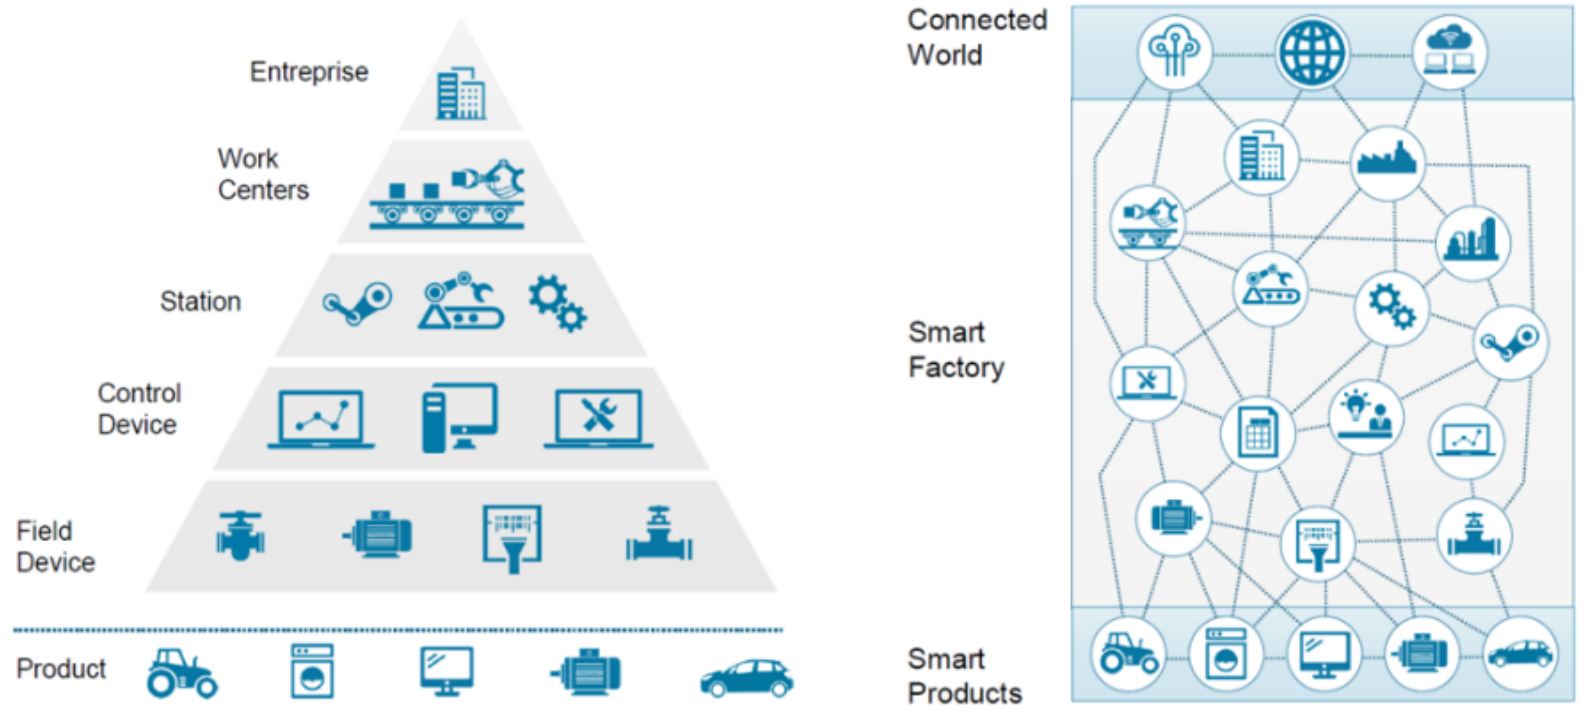
\includegraphics[width=1\textwidth]{i3-to-i4.png}
		\fonte{\citeonline{schmittner2017mtom} (adaptado).}
	\end{figure}

	Essa automatização e a troca de informações entre os ativos tem grande potencial de dar mais eficiência aos processos industriais, pois desta forma o sistema pode tomar decisões ótimas com base nas informações que lhe foram fornecidas por meio de sensores e identificadores. A visão para o futuro da produção baseado na I4.0 envolve sistemas de manufatura modulares e eficientes em cenários nos quais os produtos controlam seus próprios processos de fabricação \cite{lasi2014industryfour}.
	
	Há uma tendência global de redução do ciclo de vida do produto devido à rápida introdução de novas tecnologias para satisfazer a demanda dos clientes, especialmente em produtos eletrônicos \cite{trappey2008lifecycle}. A I4.0 se beneficia da chegada de produtos com curto ciclo de vida uma vez que o produto controla seu próprio processo de fabricação, facilitando, assim, ajustes e personalizações por parte do cliente, enquanto preserva os custos, a qualidade e o tempo de aprovisionamento (\textit{lead time}) da produção em massa.
	
	Indústria 4.0 é um conceito. Isto significa que são princípios a serem seguidos e implementados, porém o caminho para a implementação, assim como as tecnologias a serem adotadas podem ser diversos. As peculiaridades de cada indústria e de cada mercado estabelecem diferentes regras de negócios e, portanto, cada setor da indústria pode necessitar de diferentes formas e tecnologias para se implementar a I4.0 e se tornar uma fábrica inteligente. Alguns avanços tecnológicos, entretanto, são muito importantes ou essenciais para a implementação da I4.0 em qualquer sistema de manufatura, alguns deles são mostrados na \autoref{fig:tecnologias-i4}.
	
	\begin{figure}[htb]
		\centering
		\caption{Avanços tecnológicos que moldam a I4.0.}
		\label{fig:tecnologias-i4}
		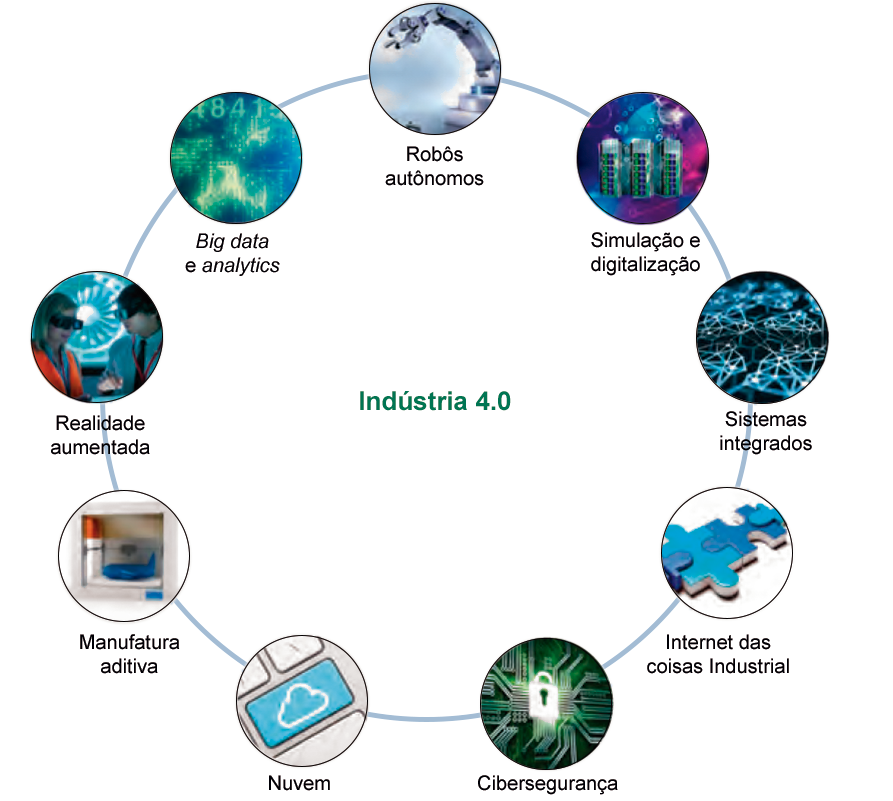
\includegraphics[width=0.8\textwidth]{tecnologias-i4.png}
		\fonte{\citeonline{russmann2015industryfour} (adaptado).}
	\end{figure}

	Após a primeira aparição do termo I4.0 na feira industrial de Hanôver em 2011, o termo ganhou significativa popularidade, principalmente no meio acadêmico e empresarial alemão. O termo foi então incentivado pelo governo alemão \cite{lasi2014industryfour, kagermann2013recommendations}, que apoiou a ideia e anunciou a Indústria 4.0 como parte integral de sua iniciativa estratégica para a indústria alemã, visando liderança em inovação tecnológica \cite{drath2014industrie} como uma abordagem para fortalecer a competitividade da indústria manufatureira alemã.	

	Por meio da iniciativa \textit{Plattform Industrie 4.0}, criada em 2013 pelo Ministério Federal da Educação e Pesquisa (\textit{Bundesministerium für Bildung und Forschung}) \cite{germany2019plattform} e com o grupo de trabalho ``Industrie 4.0 Working Group'' em comunicação com diversas associações de engenharia e indústrias alemãs, foram criados documentos oficiais como os de \citeonline{kagermann2013recommendations}, \citeonline{adolph2018roadmap} e \citeonline{bitkom2016implementation}, publicados em inglês, contendo normas e diretrizes para a implementação da I4.0. Esta iniciativa, atrelada ao entusiasmo acadêmico em torno do projeto I4.0, disseminou o conceito fora da área de língua alemã e popularizou o termo I4.0 no mundo todo como epônimo de um futuro projeto no contexto de indústrias de alta tecnologia.

	O impacto econômico dessa revolução industrial será enorme, pois a I4.0 promete uma eficiência operacional substancialmente maior, bem como o surgimento de modelos de negócios, serviços e produtos de totalmente novos \cite{hermann2016design}.
	
	Em revoluções industriais passadas, os países pioneiros a se adaptarem às drásticas mudanças de produção foram os que mais se beneficiaram e se consolidaram como potências econômicas. Na quarta revolução industrial não será diferente. Embora a mudança completa para a I4.0 possa levar 20 anos para ser concretizada \cite{russmann2015industryfour}, nos próximos anos serão estabelecidos avanços importantes que definirão os pioneiros e detentores de tecnologias dessa nova revolução. Portanto, é de interesse de cada país liderar a concorrência global a fim de se consolidar como mercado líder e fornecedor de soluções para a Indústria 4.0.

	\subsection{Modelo de Arquitetura de Referência para a Indústria 4.0}
	\label{sub:rami4}
	
	O Modelo de Arquitetura de Referência para a Indústria 4.0, abreviado RAMI4.0, consiste em um sistema de coordenadas tridimensional que descreve todos os aspectos cruciais da Indústria 4.0. Dessa maneira, inter-relações complexas podem ser divididas em grupos menores e mais simples.
	
	A \autoref{fig:rami4} mostrou a representação do RAMI4.0, especificando os itens contidos em cada eixo. A \autoref{tab:rami-eixos} fornece uma breve descrição de cada eixo do RAMI4.0.
	
	\begin{table}[htb]
		\centering
		\footnotesize
		\caption{Eixos do RAMI4.0.}
		\label{tab:rami-eixos}
		\begin{tabular}{p{3cm}p{12cm}}
			\hline
			\textbf{Eixo} &\textbf{Descrição} \\
			
			\hline
			Camadas
			& As seis camadas no eixo vertical descrevem a decomposição de um ativo em suas funcionalidades, isto é, o mapeamento virtual de um ativo. A representação em camadas se origina da tecnologia da informação e comunicação (TIC), onde as funcionalidades de sistemas complexos são comumente divididas em camadas. \\
			
			\hline
			Ciclo de vida e  Cadeia de valor
			& O eixo horizontal esquerdo representa o ciclo de vida das instalações e produtos, com base na IEC 62890 para gerenciamento do ciclo de vida. Além disso, é feita uma distinção entre ``tipos'' e ``instâncias''. Um ``tipo''~ é criado na fase de desenvolvimento e, uma vez concluída esta fase, esse tipo é liberado para a produção, servindo como modelo para uma ``instância'', que é quando produto real está sendo fabricado e possui um número de série. \\
			
			\hline
			Níveis hierárquicos
			& No eixo horizontal direito estão indicados os níveis hierárquicos da IEC 62264, a série de padrões internacionais para sistemas de TI e controle corporativos. Os níveis hierárquicos representam as diferentes funcionalidades das fábricas. Para representar o ambiente I4.0, as funcionalidades foram expandidas, incluindo adicionalmente o ``Produto'', o ``Dispositivo de campo'' e o ``Mundo conectado''. \\
			\hline
			
		\end{tabular}
		\fonte{O autor.}
	\end{table}

	A \autoref{fig:eixo-camadas} mostra o detalhamento de cada elemento do eixo Camadas do RAMI4.0 e sua associação ao modelo completo.
	
	\begin{figure}[htb]
		\centering
		\caption{(a) Representação completa do RAMI4.0 e (b) detalhamento de cada elemento do eixo ``Camadas''.}
		\label{fig:eixo-camadas}
		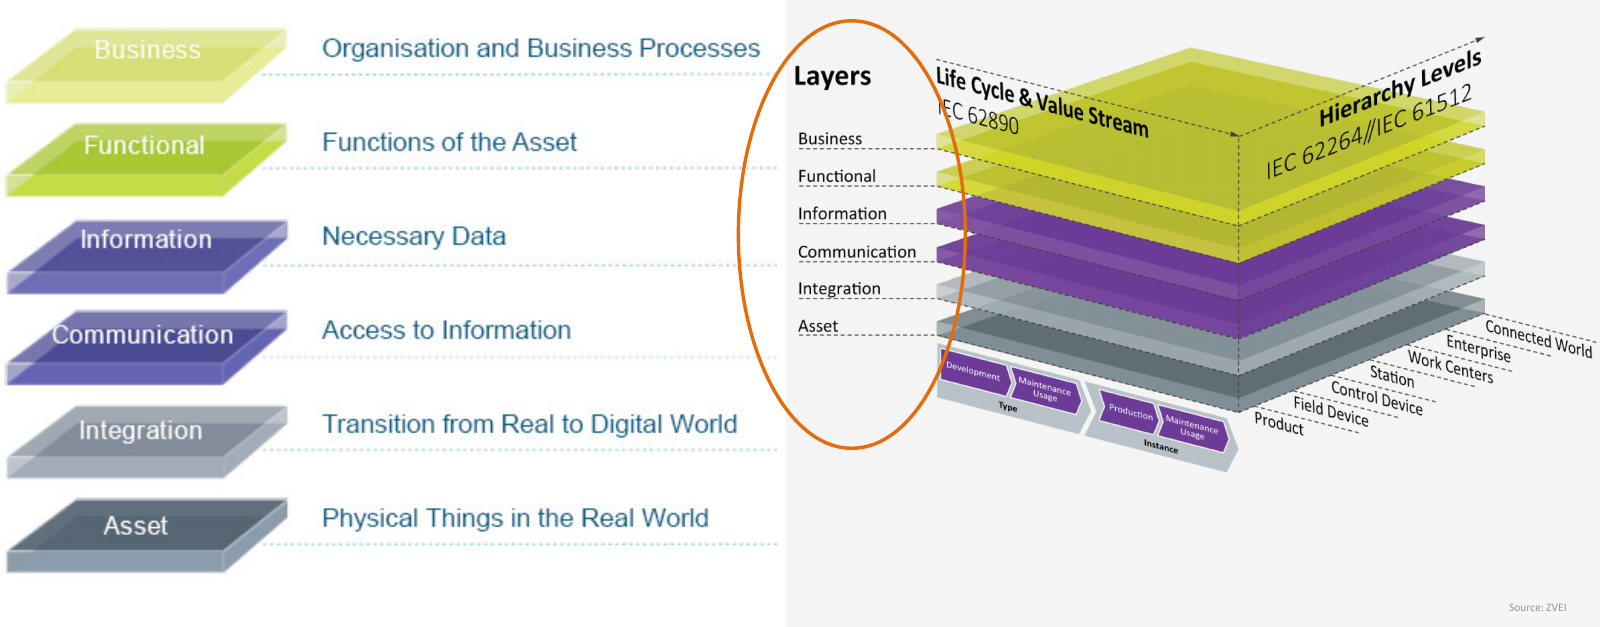
\includegraphics[width=1\textwidth]{eixo-camadas.png}
		\fonte{\citeonline{gayko2018ramistandardization} (adaptado).}
	\end{figure}

	São 6 as camadas do RAMI4.0. O propósito de cada camada, começando da mais inferior (Ativo) para a mais elevada (Regra de Negócio), é descrito a seguir \cite{bitkom2016implementation}:
	
	\begin{enumerate}
		\item \textbf{Ativo}: Representa um elemento da realidade não necessariamente físico, como, por exemplo, uma máquina, um \textit{software}, uma documentação, uma ideia, etc. O trabalhador e seu conhecimento sendo aplicado representa também um ativo. Nesta camada física estão os fornecedores de dados, ou seja, os elementos que servirão como fonte de dados. Normalmente estes dados gerados pelo ativo são extraído e monitorados para fins de controle da planta de produção. Os ativos são integrados ao meio digital através da camada de Integração. 
		
		\item \textbf{Integração}: Camada responsável pela extração e fornecimento de informações sobre os ativos para as camadas superiores. Representa a digitalização dos ativos. Cada evento no mundo real é refletido também em um evento no mundo virtual. Se a realidade mudar, esse evento então é relatado à camada de integração e os dados são atualizados no mundo virtual.
		
		\item \textbf{Comunicação}: Padronização da comunicação por meio da adoção de um formato de troca de dados uniforme entre os dispositivos. Esta camada é a responsável pela interoperabilidade entre os ativos na I4.0. Aqui ocorre a integração vertical, ou seja, a comunicação entre ativos dentro da mesma empresa. A camada de Comunicação fornece dados sobre o ativo à camada de informação.
		
		\item \textbf{Informação}: Controle dos dados do ativo. Esta camada agrega todos os dados sobre um determinado ativo e é responsável pelo gerenciamento desses dados. Na camada de informação são garantidos que os dados sejam tratados, pré-processados, armazenados e disponibilizados para os demais ativos na rede.
		
		\item \textbf{Funcional}: Contém a descrição formal de todas as funcionalidades do sistema. É também a camada responsável pela integração horizontal de ativos, ou seja, é a porta de interação entre Componentes I4.0 de diferentes empresas. Esta camada é a interface para o fornecimento de informações por meio de microsserviços para ativos fora da empresa.
			
		\item \textbf{Regra de negócio}: Contém as regras de negócio que o sistema deve seguir como, por exemplo, as condições legais e regulatórias. Esta camada também é responsável por mapear os modelos de negócios e fornecer restrições operacionais da planta de produção.
	\end{enumerate}

	Já os elementos do eixo ``Ciclo de Vida e Cadeia de Valor'' do RAMI4.0 são detalhados na \autoref{fig:eixo-ciclodevida}, juntamente com seu destaque dentro do modelo completo.
	
	\begin{figure}[htb]
		\centering
		\caption{(a) Representação completa do RAMI4.0 e (b) detalhamento do eixo ``Ciclo de Vida e Cadeia de Valor''.}
		\label{fig:eixo-ciclodevida}
		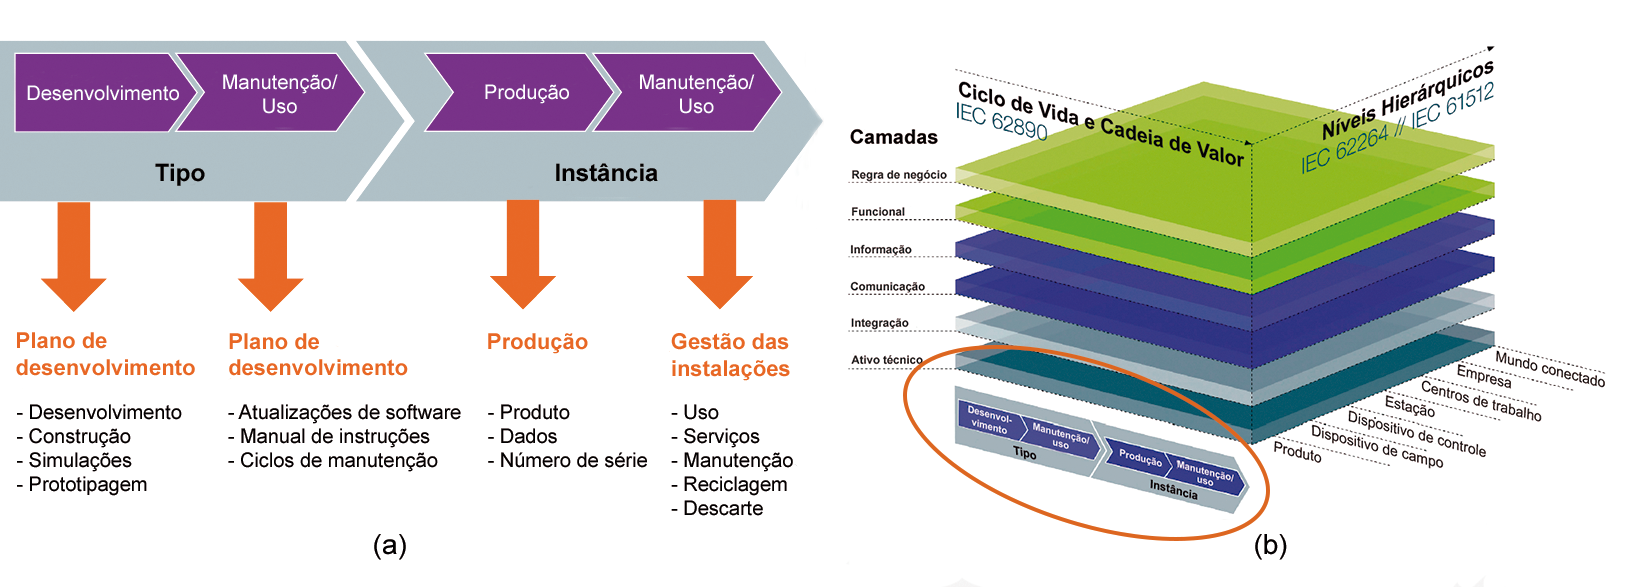
\includegraphics[width=1\textwidth]{eixo-ciclodevida.png}
		\fonte{\citeonline{gayko2018ramistandardization} (adaptado).}
	\end{figure}

	A I4.0 oferece um grande potencial de aprimoramento dos processos ao longo do ciclo de vida do produto. Este eixo fornece uma representação do estado do ativo ao longo de toda sua cadeia de suprimentos e sua cadeia de valor. 
	
	É feita a distinção fundamental entre ``tipo'' e ``instância'', cada um correspondendo a uma fase em que o produto se encontra \cite{adolphs2015rami}.
	
	Um tipo é sempre criado com uma ideia inicial, ou seja, quando um produto surge na fase de desenvolvimento. Isso abrange o comissionamento, desenvolvimento e testes até a produção inicial de amostras e protótipos \cite{adolph2018roadmap}. 
	
	Com a conclusão de todas as etapas de testes e validação, o tipo é liberado para produção em série. A partir de então, novos produtos podem ser instanciados com base neste tipo validado. 
	
	Com a fabricação do produto, instâncias são geradas. Cada produto fabricado representa uma instância de um determinado tipo e recebe um número de série exclusivo.
	
	As melhorias sobre um produto feitas pelo fabricante refletem em um novo tipo, que por sua vez pode ser usado para fabricar novas instâncias, acompanhando, assim, o ciclo de vida do produto.

	O último eixo descrito, ``Níveis Hierárquicos'', do RAMI4.0 é apresentado na \autoref{fig:eixo-niveishierarquicos}. Nesta representação, o último nível -- ``Mundo conectado'' (não representado no detalhamento à direita) -- é a interconexão e interoperabilidade entre as mais de diversas empresas, que por sua vez possuem todas as demais camadas inferiores listadas.
	
	\begin{figure}[htb]
		\centering
		\caption{(a) Representação completa do RAMI4.0 e (b) detalhamento do eixo ``Níveis Hierárquicos do RAMI4.0''.}
		\label{fig:eixo-niveishierarquicos}
		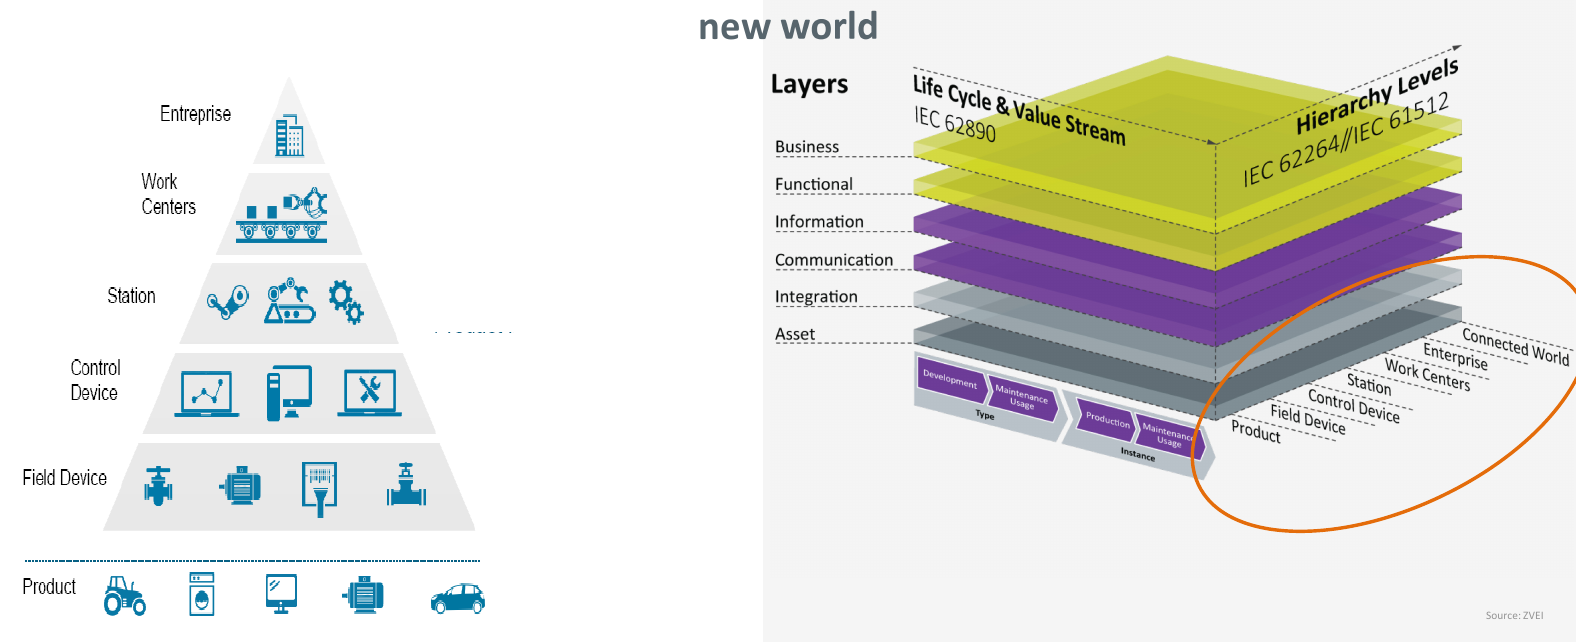
\includegraphics[width=1\textwidth]{eixo-niveishierarquicos.png}
		\fonte{\citeonline{gayko2018ramistandardization} (adaptado).}
	\end{figure}

	Este eixo representa as diferentes funcionalidades das fábricas e descreve a integração dos sistemas empresariais de controle \cite{pisching2018arquitetura}.
	
	Este eixo é baseado em uma reformulação da IEC 62264, que é a série de padrões internacionais para sistemas de TI e controle corporativos \cite{hankel2015rami}, e faz uma alusão à pirâmide da automação industrial da ISA-95.
	
	Os níveis hierárquicos representam as diferentes funcionalidades das fábricas. Para representar o ambiente I4.0, as funcionalidades foram expandidas além da IEC 62264, que já possui os níveis ``Dispositivo de controle'', ``Estação de trabalho'', ``Centros de trabalho'' e ``Empresa''.
	
	Para a representação do ambiente I4.0, foi adicionado o nível ``Produto'' na posição mais inferior para descrever funcionalidades relacionadas ao produto da manufatura, o nível ``Dispositivo de campo'', com considerações a nível funcional sobre dispositivos de campo inteligentes, e o nível ``Mundo conectado'' na posição mais superior para descrever o grupo de fábricas e a colaboração entre empresas, fornecedores de componentes, clientes, etc. 

	Dentro dos três eixos, todos os aspectos cruciais da I4.0 podem ser mapeados, permitindo que os ativos sejam classificados devidamente de acordo com o modelo. Os conceitos altamente flexíveis da I4.0 podem, assim, ser descritos e implementados usando o RAMI4.0. O modelo de arquitetura de referência permite a migração passo a passo do presente estado da indústria para o mundo da Indústria 4.0.
	
	\subsection{Asset Administration Shell}
	
	Um ativo é qualquer coisa que precise ser conectada para agregar valor a um processo industrial \cite{bader2019aas}, ou seja, todos os itens que têm valor em um caso de uso específico. Na I4.0, isso pode ser um produto físico, uma peça de equipamento, um \textit{software} ou documentos como plantas, contratos, pedidos, etc.
	
	No paradigma da I4.0, cada ativo é encapsulado por uma camada (ou casca) de administração. Esta casca de administração do ativo técnico é denominada \textit{``Asset Administration Shell''} (AAS). O AAS é a representação da parte virtual/digital de um ativo no mundo I4.0 \cite{ye2019aas}.
	
	Fazendo uma associação ao RAMI4.0, o AAS engloba as camadas digitais, sendo elas: Regra de Negócio, Funcional, Informação e Comunicação; parte da camada Integração também é contemplada pelo AAS, já que essa é a conexão entre o ativo e o meio virtual. Tal associação é representada pela \autoref{fig:aas-rami}.

	\begin{figure}[htb]
		\centering
		\caption{Representação do AAS como a parte virtual do Componente I4.0.}
		\label{fig:aas-rami}
		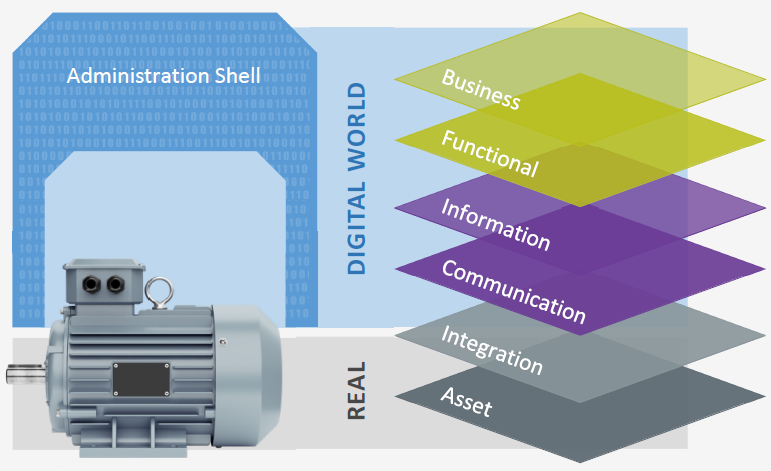
\includegraphics[width=0.8\textwidth]{aas-rami.png}
		\fonte{\citeonline{gayko2018ramistandardization} (adaptado).}
	\end{figure}
		
	O AAS consiste em vários submodelos nos quais são descritas todas as informações e funcionalidades de um determinado ativo, incluindo suas características, propriedades, condição, parâmetros, dados de medições e capacidades \cite{bader2019aas}. A \autoref{fig:aas-submodelos} exemplifica um AAS como sendo uma ``casca'' que engloba o ativo, esta casca contém informações relevantes do ativo em forma de ``submodelos''.
	
	\begin{figure}[htb]
		\centering
		\caption{Exemplificação de um AAS para um servomotor, incluindo os submodelos de identificação, dados técnicos, dados operacionais e documentação.}
		\label{fig:aas-submodelos}
		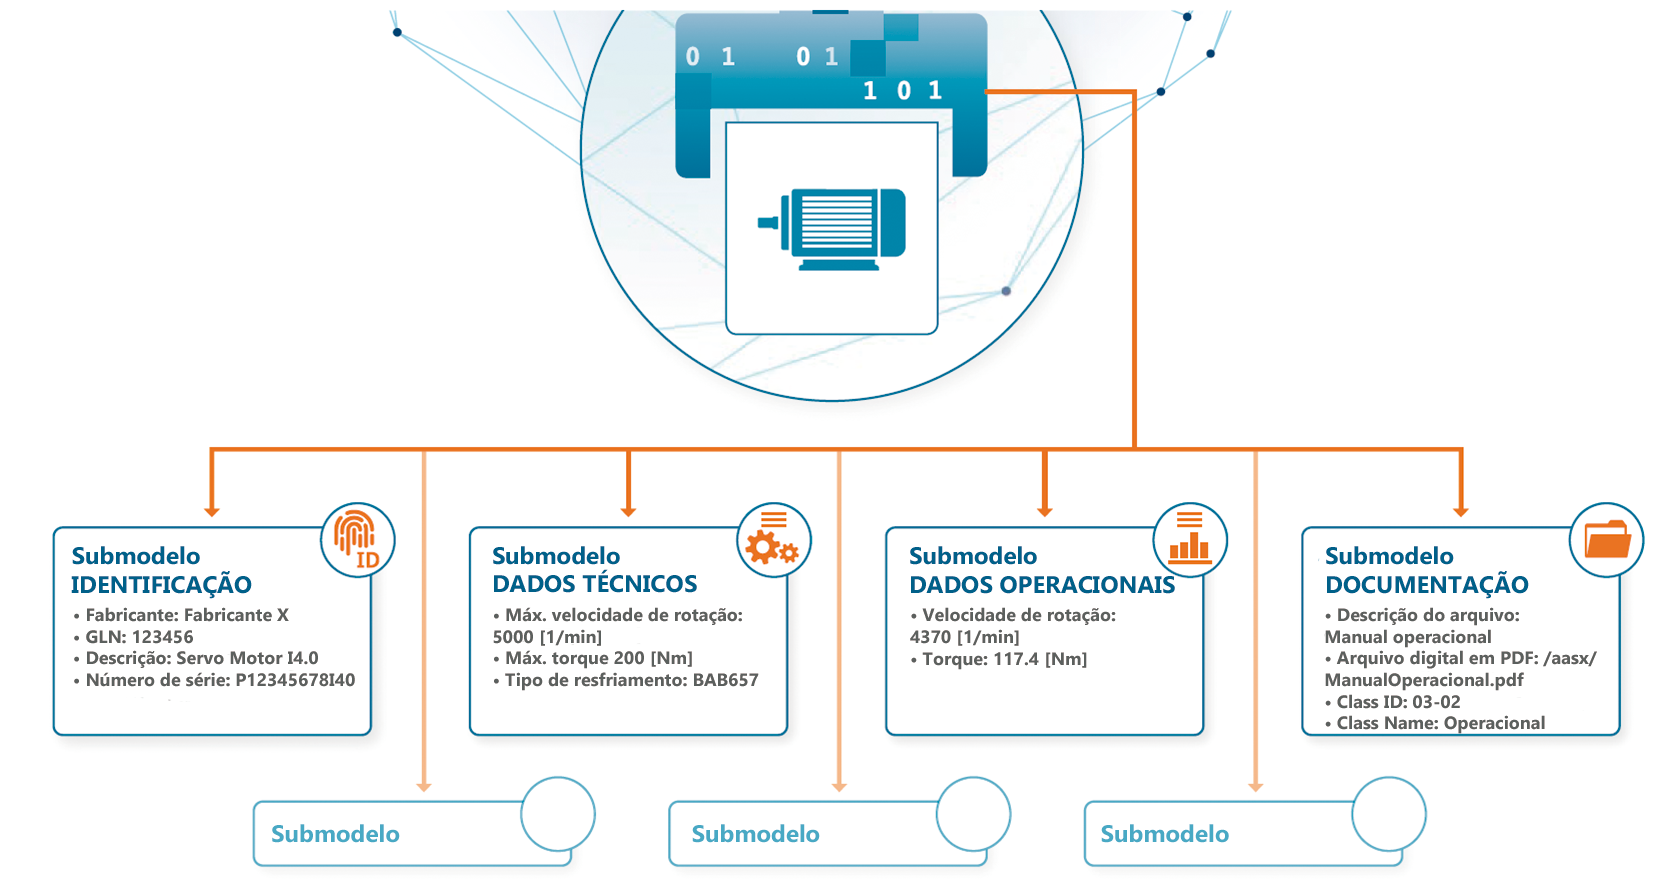
\includegraphics[width=1\textwidth]{aas-submodelos.png}
		\fonte{\citeonline{bader2019aas} (adaptado).}
	\end{figure}

	Os submodelos são unidades básicas de organização dentro de um AAS que agregam informações semelhantes. Eles são divididos em dois tipos \cite{plattform2019detailsaas}: submodelos básicos e submodelos livres \cite{bader2019aas}.
	
	Os submodelos básicos são unidades de organização que se aplicam a muitos ou todos os ativos dentro do mundo I4.0. Já os submodelos livre são acertados entre os parceiros na cadeia de suprimentos e possuem um uso específico para um determinado produto.
	
	O AAS é um elo entre os ativos reais e seus correspondentes digitais no mundo conectado. A \autoref{fig:aas-conexao} ilustra a comunicação entre diferentes AASs em um ambiente de manufatura I4.0 sob uma ontologia comum.
	
	\begin{figure}[htb]
		\centering
		\caption{Comunicação entre AASs de componentes I4.0.}
		\label{fig:aas-conexao}
		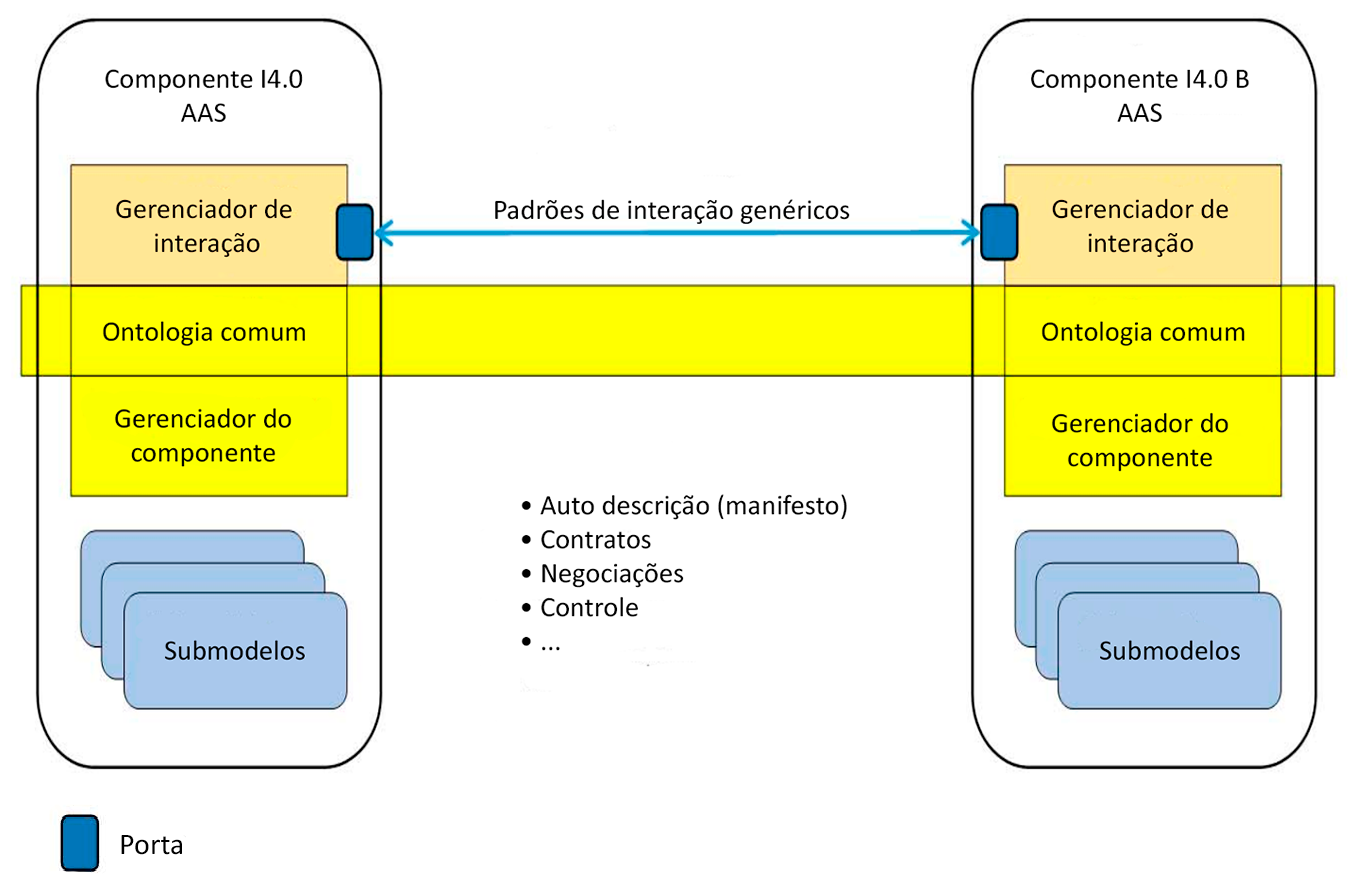
\includegraphics[width=1\textwidth]{aas-conexao.png}
		\fonte{\citeonline{marcon2018asset} (adaptado).}
	\end{figure}

	Dentro da I4.0, todos os ativos possuem um AAS com capacidade de comunicação com outros dispositivos. O conjunto Ativo-AAS, que é o objeto real encapsulado pelo \textit{Asset Administration Shell}, é denominado ``Componente I4.0''.
	
	A integração dos ativos, representada pelos Componentes I4.0, em um nível funcional requer uma descrição padronizada das funções (ou capacidades) dos ativos em questão. A padronização de submodelos para descrever detalhadamente cada função pode ser usada para definir requisitos para a fabricação de produtos \cite{bedenbender2017aasexamples}. A \autoref{fig:submodelos} mostra um exemplo de detalhamento de funções de um ativo.
	
	\begin{figure}[htb]
		\centering
		\caption{Detalhamento de funções no AAS por meio de submodelos.}
		\label{fig:submodelos}
		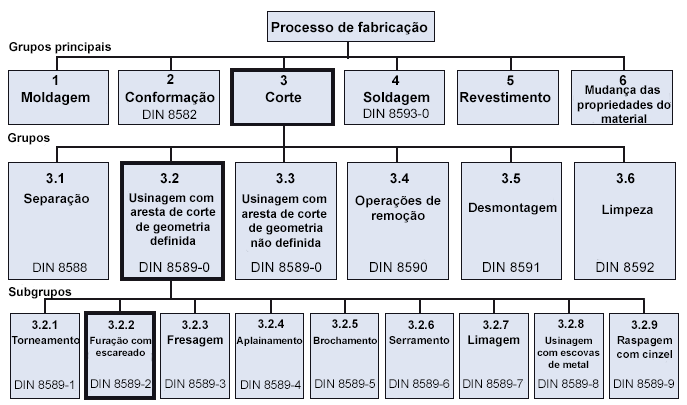
\includegraphics[width=1\textwidth]{submodelos.png}
		\fonte{\citeonline{bedenbender2017aasexamples} (adaptado).}
	\end{figure}

	No ambiente de manufatura baseado na I4.0, o produto descreve os requerimentos necessários para sua fabricação e então esses requerimentos são comparados com as descrições das funções das máquinas disponíveis. Portanto, a seleção de um ativo é otimizada, baseando-se nos requerimentos do produto e nas descrições das funções dos ativos.
	
	Desta forma, um Componente I4.0 representa todos os elementos necessários para a efetiva interoperabilidade entre ativos no mundo conectado, inclusive os seus próprios requisitos, suas regras de negócio, limitações técnicas e todas as demais características que se relacionem ao ativo e sua interação com o ambiente.
	
\section{Logística \& Cadeia de Suprimentos}
\label{sec:logistica}
	
	A logística é o processo de planejamento, implantação e controle do fluxo de mercadorias, serviços e informações relativas desde o ponto de origem até o ponto de consumo de forma eficiente e eficaz com o propósito de atender as exigências dos clientes \cite{cscmp2013supplychainglossary}. Essa definição sugere a logística como um processo, o que significa que inclui todas as atividades importantes para a disponibilização de bens e serviços aos consumidores quando e onde estes quiserem adquiri-los \cite{ballou2006cadeiasuprimentos}.
	
	A logística é a essência do comércio \cite{ballou2006cadeiasuprimentos}, ela contribui para que pessoas não mais sejam obrigadas a viver perto das fontes de produção e possam trocar informações e mercadorias com outras regiões de forma efetiva, contribuindo decisivamente para melhorar o padrão econômico de vida geral. 
	
	A logística moderna envolve primariamente o compartilhamento de dados. A logística da informação lida com o fluxo de informações entre humanos e/ou máquinas dentro ou entre organizações \cite{haftor2009information}, que se agrupam formando uma rede de criação de valor por meio de informações. A Logística da Informação é intrinsecamente relacionada a processos de gestão da informação e tecnologias de informação.
	
	A cadeia de suprimentos (CS), por outro lado, é um conceito mais amplo. A CS é onde a logística é exercida. São as partes necessárias para dar suporte ao pedido de um cliente, desde o produtor até o consumidor final. A gestão da cadeia de suprimentos tem como alvo a orquestração de todas as partes envolvidas por meio de uma logística integrada de forma a otimizar ao máximo o processo de fornecimento de um produto, serviço ou informação.
	
	A ideia de uma CS simples envolve fornecedor, produtor e cliente \cite{hugos2018supplychain}, porém conceitos modernos estendem a noção de uma CS, passando a incluir diversos outros fornecedores de serviços em áreas como logística, finanças, \textit{marketing} e desenvolvimento; que, mediante coordenação e colaboração, criam oportunidades para melhoria dos custos ou serviços ao consumidor. A \autoref{fig:cadeia-de-suprimentos} exemplifica a inter-relação das partes em uma cadeia de suprimentos estendida.
	
	\begin{figure}[htb]
		\centering
		\caption{Exemplo de cadeia de suprimentos estendida.}
		\label{fig:cadeia-de-suprimentos}
		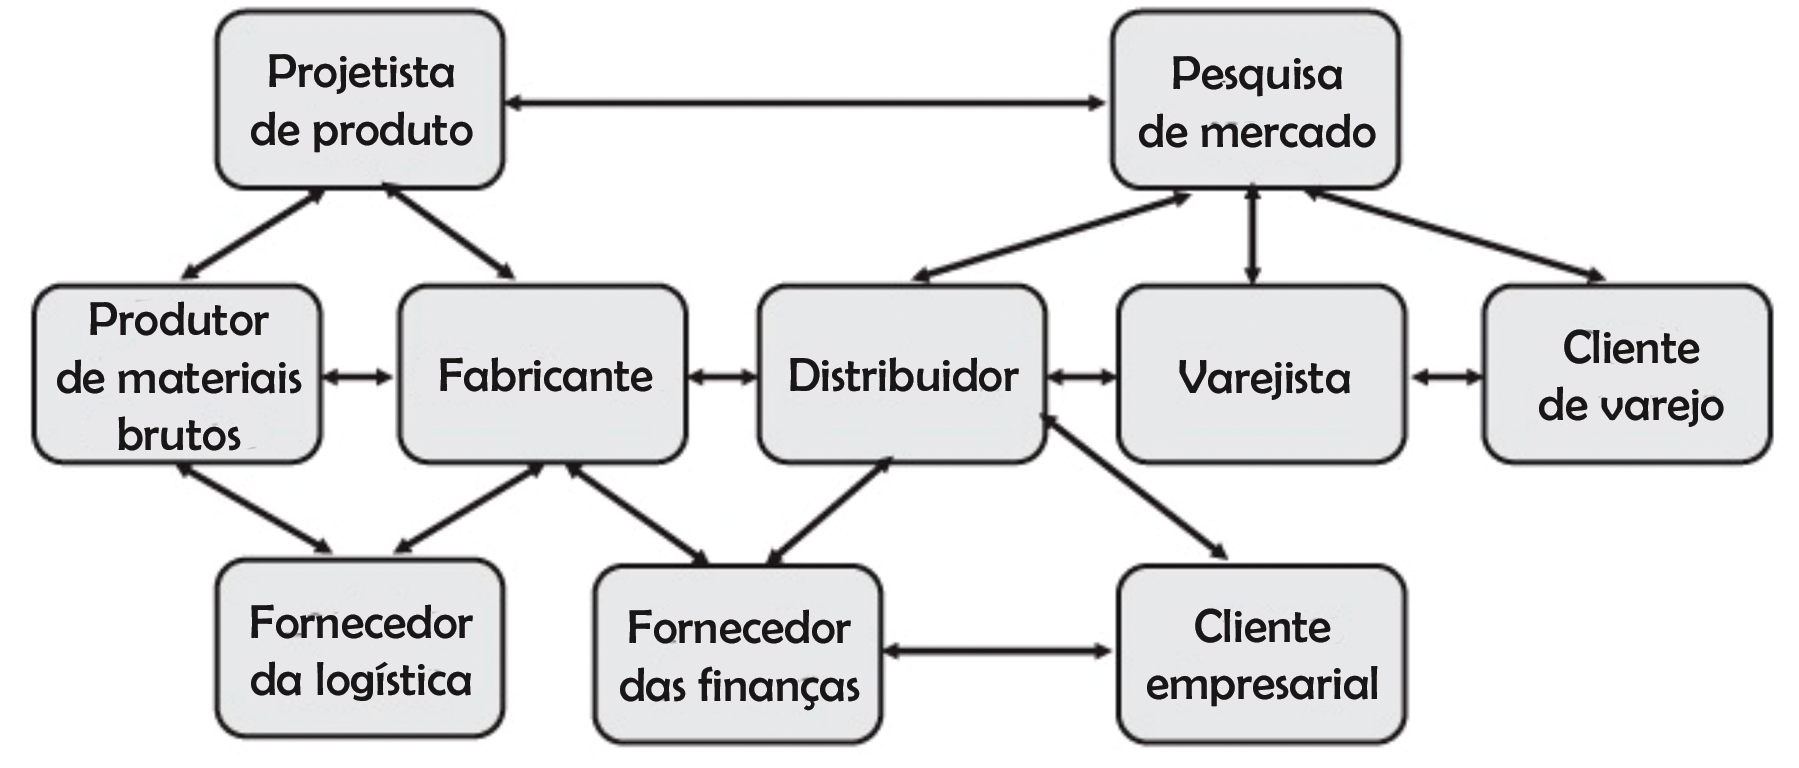
\includegraphics[width=1\textwidth]{cadeia-de-suprimentos.png}
		\fonte{\citeonline{hugos2018supplychain} (adaptado).}
	\end{figure}
	
	Além do eficiente fluxo de materiais e produtos dentro da CS, é imprescindível a manutenção de um canal para troca de informações entre as partes em uma CS, pois sem uma adequada comunicação, gerentes podem acidentalmente tomar decisões supostamente racionais, porém que afetam negativamente outros líderes da cadeia, como o efeito chicote \cite{lee1997bullwhip}, que é a distorção da percepção da procura de um produto que vai se ampliando ao longo da cadeia de suprimentos. Erros de comunicação desse tipo podem acarretar problemas como o aumento do custo de transporte, o elevado tempo de aprovisionamento ao cliente e o desgaste no relacionamento com os fornecedores.
	
	Ao longo da cadeia de suprimentos pode-se observar processos que agregam valor ao produto em desenvolvimento. As etapas de transformação do produto com adição de valor ao longo da CS também podem ser definidas como Cadeia de Valor (CV).
	
	Uma CV é um conjunto de atividades que empresas de um setor específico desempenham a fim de entregar um produto ou serviço que tenha algum valor perceptível para o mercado \cite{porter1985competitiveadvantage}. A ideia da CV é baseada na agregação de valor ao produto a cada processo de transformação ocorrido, processo esse que envolve a aquisição e consumo de recursos (mão de obra, materiais, equipamentos, instalações, administração, etc). \citeonline{porter1985competitiveadvantage} classifica a CV em duas categorias de atividades que agregam valor ao produto: as atividades primárias e as atividades de apoio (vide \autoref{fig:porter-cadeia-de-valor}).
	
	\begin{figure}[htb]
		\centering
		\caption{Cadeia de valor de Porter.}
		\label{fig:porter-cadeia-de-valor}
		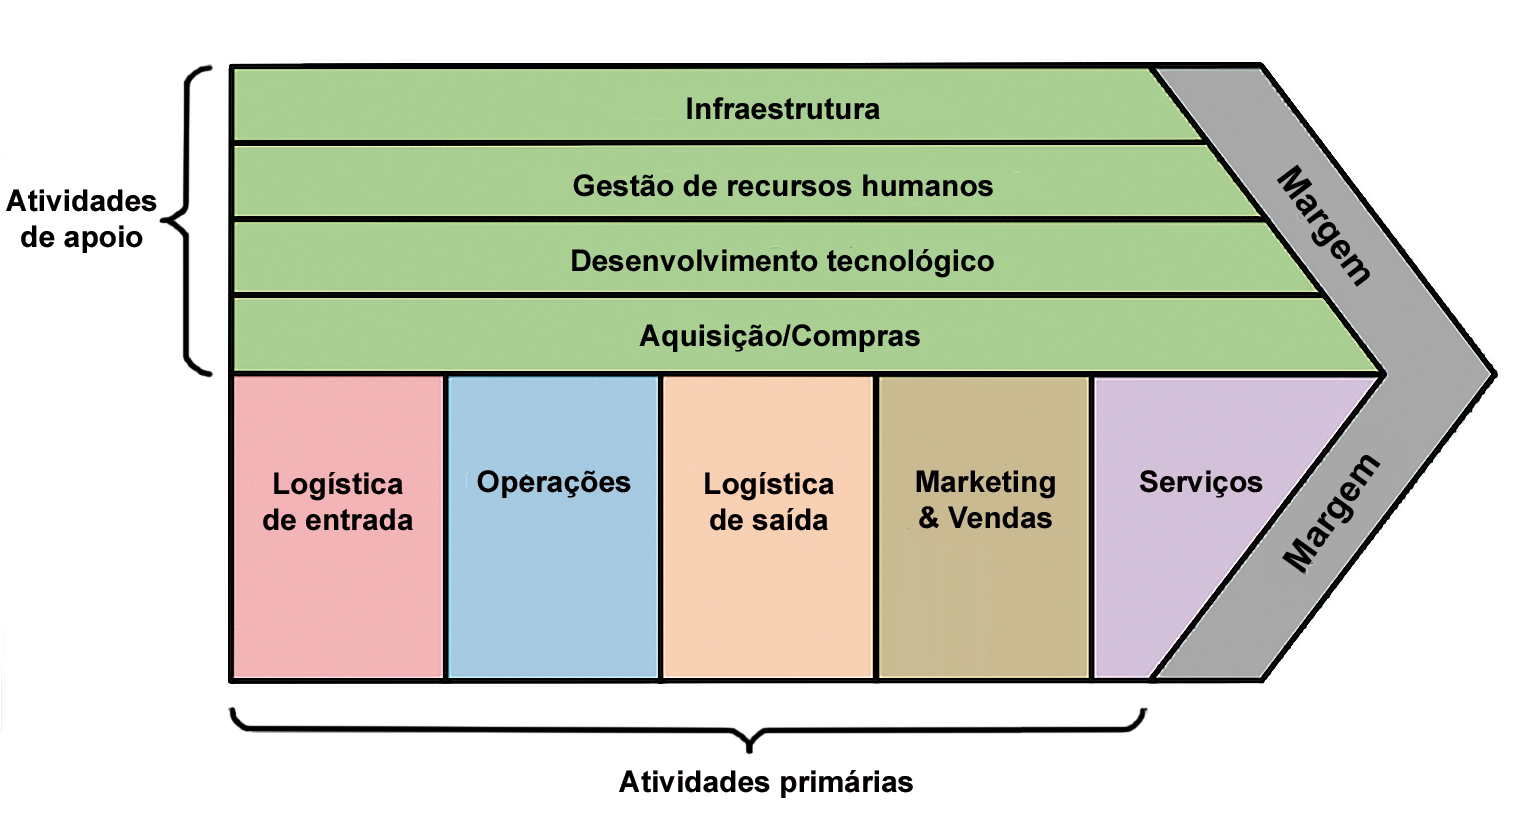
\includegraphics[width=1\textwidth]{porter-cadeia-de-valor.png}
		\fonte{\citeonline{porter1985competitiveadvantage} (adaptado).}
	\end{figure}
	
	As CVs estão focadas em fornecer o máximo valor ao cliente (valor perceptível) com o menor custo e, portanto, é um indicador para a competitividade da empresa. Com o crescente acirramento da competição entre as empresas, essas devem procurar novas formas de agregar mais valor perceptível aos seus produtos, sendo isto em forma de redução de preço, aumento de qualidade, suporte ou qualquer outra nova funcionalidade.
	
	Outra forma de agregação de valor está no princípio de valor compartilhado, que envolve a geração de valor econômico de forma a criar também valor para a sociedade como um todo \cite{porter2011valorcompartilhado} com o enfrentamento de suas necessidades e desafios. Esta necessidade de valor compartilhado parte da percepção generalizada de que empresas prosperam às custas da depreciação da comunidade que as cercam. Soluções que visem o aumento das condições de trabalho, a maior racionalidade e eficiência no tratamento dos recursos naturais necessários para sua atividade e outras formas de balancear o \textit{trade-off} entre eficiência econômica e progresso social são estratégias para se recuperar a legitimidade e a percepção de valor pela sociedade da atividade empresarial.
	
	\subsection{Logística 4.0}
	
	Com o entusiasmo acadêmico sobre o tema Indústria 4.0 surgido a partir de 2011, diversas novas linhas de pesquisa derivaram do conceito de I4.0. Uma dessas vertentes é relacionada aos novos desafios tecnológicos na logística e por vezes é denominada ``Logística 4.0''. Estes novos desafios tecnológicos são relacionados primariamente ao intenso uso das Tecnologias de Informação e Comunicação (TIC) e de Internet das Coisas Industrial (IIoT) \cite{barreto2017industry}.
	
	A inserção dessas novas tecnologias ao escopo de estudo da logística acarreta em novos desafios como a alta necessidade de transparência dos processos (visibilidade ao longo da cadeia de suprimentos) e o controle de integridade (produtos certos, no tempo, lugar, quantidade, condição e preço certos) \cite{barreto2017industry}.

	As cadeias de suprimentos atuais podem ser extremamente grandes e complexas (alta interdependência entre as partes) e, portanto, sem uma correta gestão, podem levar à tomada de decisões não ótimas por parte dos gestores humanos. Por esses aspectos, este setor pode ser um dos primeiros a se adaptar a esta nova forma de organização da Indústria 4.0 (ou da Logística 4.0), tornando os processos cada vez mais automatizados a fim de se atender os novos requisitos da sociedade moderna.

	Dentro da CS, identificadores individuais podem ser usados a fim de se implementar a conectividade de objetos e informações requeridos no contexto da I4.0. 
	
	A tecnologia de RFID (\textit{Radio-Frequency IDentification}) permite criar uma identificação única para um objeto, onde a etiqueta RFID é um pequeno \textit{chip} que pode ser acoplado e incorporado a um produto e assim armazena um código de identificação único, assim como outras informações relevantes, que podem ser transmitidas sem fio via rádiofrequência. O RFID se mostra como uma alternativa ao tradicional código de barras e o \textit{QR code}. A utilização de identificadores individuais é comum para aplicação de conceitos da I4.0 \cite{alyahya2016rfidwarehousing, vlachos2014rfidimpact, fan2015inventory, bibi2017rfidfood}, pois permite a identificação de cada coisa na rede e possibilita a troca de informações autônomas.
	
	A Logística 4.0, portanto, estabelece uma série de paradigmas que empresas atuando no ramo logístico deverão seguir nos próximos anos para se manterem competitivas. Conceitos de operação como o intercâmbio de informações instantâneas, soluções automatizadas e análise de dados em tempo real abrem caminhos para novos modelos de negócios \cite{strandhagen2017logistics}, que se tornarão essenciais na eficiência em logística moderna.

	
\section{Ciclo de vida do produto}
	
	O conceito de ciclo de vida do produto foi elaborado em meados da década de 1960 com o propósito de criar um modelo que fosse capaz de explicar o sucesso ou fracasso de um produto introduzido no mercado, sendo capaz também de identificar momentos certos para modificar estratégias de preço, fabricação e quando o produto deve ser descontinuado \cite{cao2012lifecycle}. O modelo inicialmente desenvolvido por \citeonline{levitt1965lifecycle} mostra o padrão de produtos na história passando por quatro estágios bem definidos: desenvolvimento de mercado, crescimento, maturidade e declínio, conforme observado na \autoref{fig:product-life-cycle}.
	
	\begin{figure}[htb]
		\centering
		\caption{Estágios do ciclo de vida do produto.}
		\label{fig:product-life-cycle}
		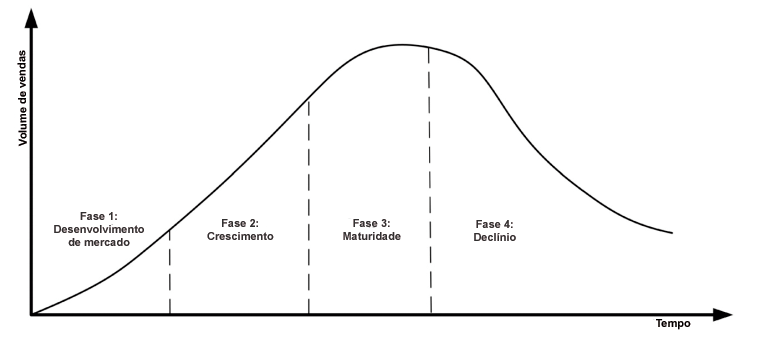
\includegraphics[width=1\textwidth]{product-life-cycle.png}
		\fonte{\citeonline{levitt1965lifecycle} (adaptado).}
	\end{figure}
	
	Vista a tendência global de redução do ciclo de vida do produto devida a rápida taxa de introdução de novas tecnologias para satisfazer a demanda dos clientes, especialmente no mercado de produtos eletrônicos \cite{trappey2008lifecycle}, novas versões de modelos de ciclo de vida do produto vêm sendo elaboradas considerando outros aspectos de mercado e não somente sob a visão da área de \textit{Marketing}. Por vezes, estudos recentes envolvendo ciclo de vida são denominados ``engenharia do ciclo de vida do produto'' (E-CVP) \cite{cao2012lifecycle} e levam em consideração fatores não abordados nos modelos originais como, por exemplo, a fase de pesquisa e desenvolvimento, a retroalimentação de dados, assim como o descarte e reciclagem do produto. Sempre tendo como objetivo auxiliar na tomada de decisões para o sucesso de um produto no mercado.
	
	A \autoref{fig:ciclo-de-vida-extensao} mostra um modelo de ciclo de vida do produto com elementos que incluem a fase de desenvolvimento e a renovação do produto. A renovação do produto e a decorrente extensão de sua vida é essencial, pois mantém o produto no mercado na forma de novas versões e, assim, amplia as receitas mediante ações estratégicas para agregação de valor. O modelo do ciclo de vida e os elementos presentes sempre irão variar conforme a natureza do produto e tipo de mercado consumidor onde o mesmo está inserido.
	
	\begin{figure}[htb]
		\centering
		\caption{Modelo de ciclo de vida do produto com renovação do produto.}
		\label{fig:ciclo-de-vida-extensao}
		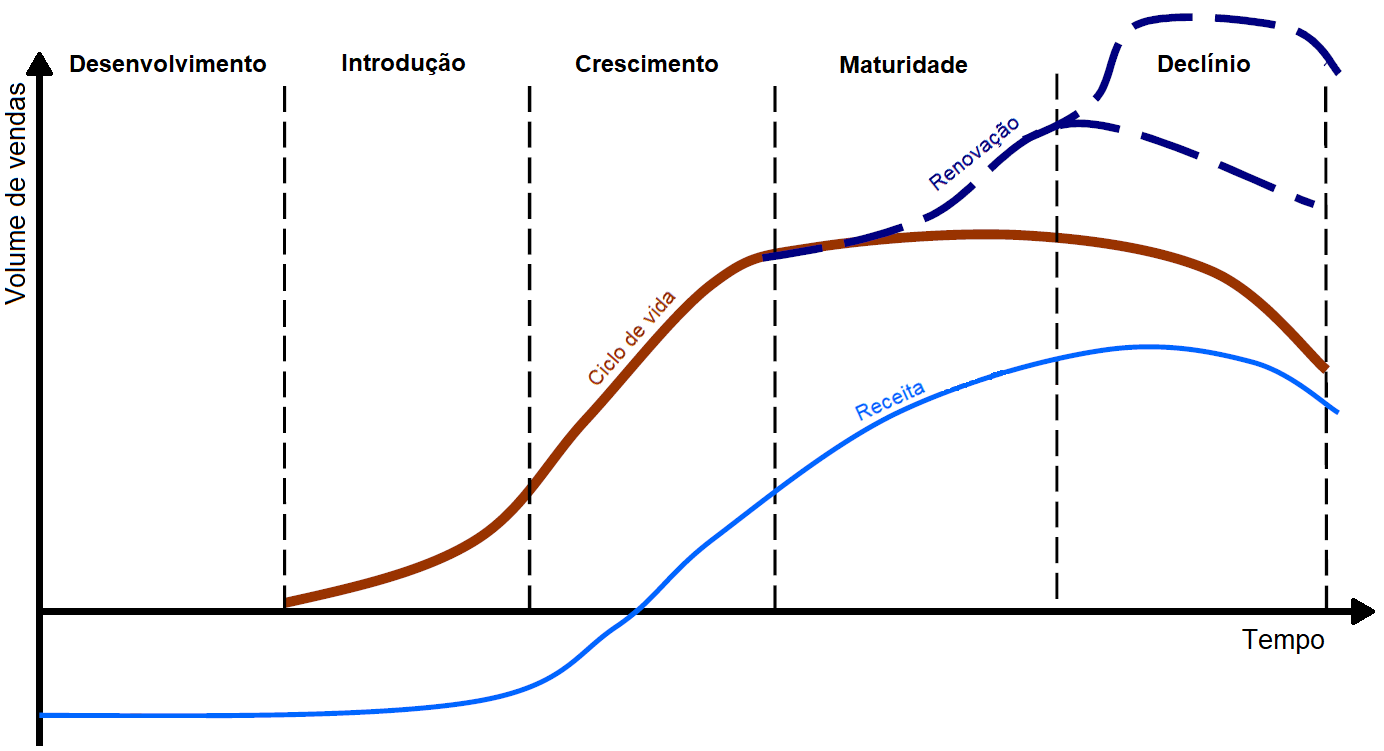
\includegraphics[width=1\textwidth]{ciclo-de-vida-extensao.png}
		\fonte{\citeonline{liu2010marketingrisk} (adaptado).}
	\end{figure}
	
	A gestão do ciclo de ciclo de vida do produto (GCVP) refere-se ao gerenciamento de um ativo ao longo dos estágios típicos de sua vida útil (vide \autoref{fig:product-life-cycle}). Esta gestão dentro dos estágios mencionados pode se referir, por exemplo, à fabricação, comercialização, uso ou qualquer outra fase do ciclo de vida em que o produto se encontra. 
	
	A GCVP tem como finalidade auxiliar gestores na tomada de decisões de negócios por meio de estratégias como políticas de preços, expansão de mercado, retirada do produto ou inserção de novas versões, etc. A função da GCVP não é gerenciar apenas um produto, mas gerenciar de maneira integrada todas as partes, assim como o portfólio de produtos da empresa \cite{stark2015lifecycle}.
	
	Em nível mais alto, o objetivo do GCVP é aumentar as receitas do produto, reduzir os seus custos relacionados, maximizar o valor do portfólio e maximizar o valor dos produtos atuais e futuros para clientes e acionistas \cite{stark2015lifecycle}.
	
	Mais recentemente, novas propostas de modificações de processos industriais por meio da GCVP aparecem como formas de se agregar mais valor ao produto/serviço considerando os ciclos de vida do produto cada vez mais curtos. A Indústria 4.0 e a Logística 4.0 surgem com novas formas de abordagem da gestão do ciclo de vida do produto, considerando as mais novas necessidades do produto e de seus respectivos consumidores.

\section{Memória digital do produto}

	O termo ``Memória Digital do Produto'' (MDP) surgiu pela primeira vez em 2007 por meio de um boletim de notícias de tecnologia de uma empresa alemã fabricante de conectores elétricos e eletrônicos \cite{wahlster2007digitalmemory}. À época, o termo foi tratado com analogia a um diário, que mantinha todas as informações do produto ao longo de seu ciclo de vida.
	
	Hoje, o conceito na literatura se refere a sistemas que permitem a coleta de dados em todas as fases do ciclo de vida do produto para a distribuição e/ou análise. Os dados de interesse do produto podem ser relativos a qualquer fase do produto ao longo de sua cadeia de suprimentos, o que abrange dados de produção individual, de montagem, de distribuição, de uso por parte do consumidor, etc. A \autoref{fig:mdp} ilustra o conceito de MDP.
	
	\begin{figure}[htb]
		\centering
		\caption{Coleta de dados do produto ao longo da cadeia de valores.}
		\label{fig:mdp}
		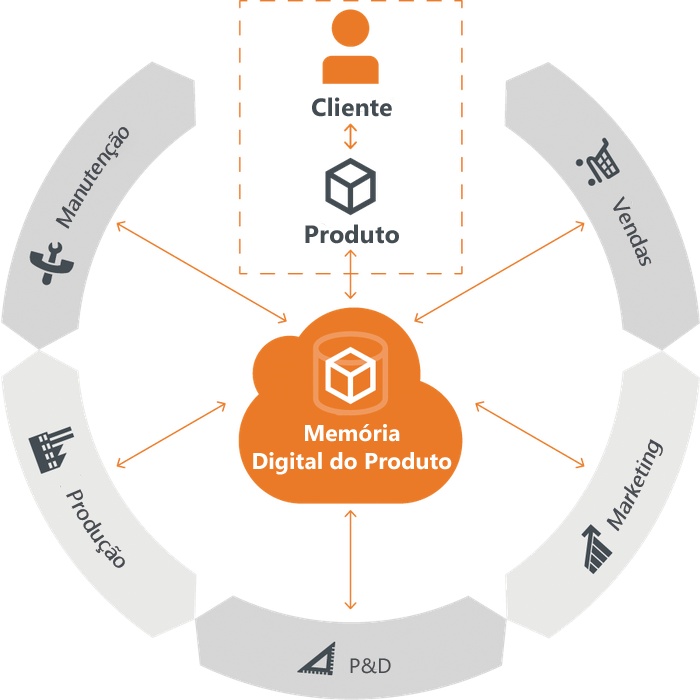
\includegraphics[width=0.6\textwidth]{mdp.png}
		\fonte{\citeonline{zuhlke2020digitalmemory} (adaptado).}
	\end{figure}
	
	Sua relevância está no fato da tendência de produtos novos apresentarem ciclos de vida cada vez mais curtos e devido ao fato das cadeias de suprimentos apresentarem redes cada vez mais complexas, com múltiplos fornecedores e clientes. Com isso, a MDP manteria registros digitais do ciclo de vida dos produtos, faria o monitoramento constante do seu estado atual e realizaria o rastreamento de sua posição. Segundo \citeonline{wahlster2007digitalmemory}, o acesso a essas informações pelas partes interessadas seria de vital importância na competitividade de empresa produtoras e de comércio, além de abrir novas proteções em relação à pirataria.
	
	Os produtos que são produzidos no cenário de Indústria 4.0 podem ser equipados com a MDP e por meio dela extrair e armazenar informações relevantes de eventos ocorridos ao longo do ciclo de vida do produto a fim de fornecer serviços a todo o ambiente com o qual o produto se relaciona \cite{brandherm2011productmemory}. A MDP fornece também uma forma de rastreabilidade, uma vez que pode armazenar informações geoespaciais do ativo ao longo do tempo.
	
	Implementações de uma memória com informações sobre produto ao longo de sua cadeia de suprimentos é importante, pois torna possível acessar e utilizar informações do mundo real providenciada por diferentes fontes para o potencial benefício das partes interessadas naquele produto \cite{brandherm2011productmemory}, como, por exemplo, fabricantes, transportadores, varejistas e consumidores. E também no pós-venda, onde a MDP continua a ser disponibilizada e ativa, dando a possibilidade ao consumidor de ainda manter contato com cada elo da cadeia de suprimentos e se beneficiar de serviços individuais que se acumulam na memória \cite{brandherm2011productmemory}.
	
\section{Arquitetura orientada a serviços}
\label{sec:webservices}
	
	Arquitetura Orientada a Serviços (SOA) é um estilo de projeto de \textit{software} em que serviços são disponibilizados a outros sistemas por meio de um protocolo de comunicação comum em uma rede \cite{bell2008soa}. Um serviço é uma unidade de funcionalidade que pode ser fornecida/acessada remotamente. A SOA se destina a ser independente de fornecedores, produtos e tecnologias.
	
	Para quem consome um serviço, a abordagem é como uma caixa preta, o que significa que o consumidor não sabe ou não precisa estar ciente do funcionamento interno deste serviço, sendo apenas o seu resultado relevante. Os serviços representam uma lógica de fornecimento de resultados. É uma abstração de problemas, ou seja, toda a complexidade interna inerente aos serviços pode ser abstraída/desconsiderada pelos consumidores dos serviços.
	
	Dentro do mundo da Indústria 4.0 e de sistemas produtivos, a SOA é uma abordagem que traz novas perspectivas uma vez que se estabelece um conjunto de princípios para uma arquitetura de sistema autônomo e interoperável \cite{candido2009soa}, que tem por objetivo aumentar a eficiência, agilidade e produtividade de um sistema por meio da adoção generalizada do conceito de serviços \cite{souit2013soa}.
	
	Os serviços dentro do ambiente de manufatura encapsulam as funcionalidades necessárias, ocultando todas as heterogeneidades das partes do sistema, permitindo, desta forma, características de flexibilidade, confiabilidade e fácil implementação de	soluções \cite{groba2008soa}.
	
	A SOA dentro do meio industrial permite que um sistema atue como \textit{middleware}, ou seja, uma camada ou componente de \textit{software} que integra os diferentes aplicativos em um sistema. A \autoref{fig:middleware} ilustra como se dá a interconexão entre os elementos do sistema com e sem um \textit{middleware}.
	
	\begin{figure}[htb]
		\centering
		\caption{Interconexão entre os elementos do sistema (a) com um \textit{middleware} e (b) sem um \textit{middleware}.}
		\label{fig:middleware}
		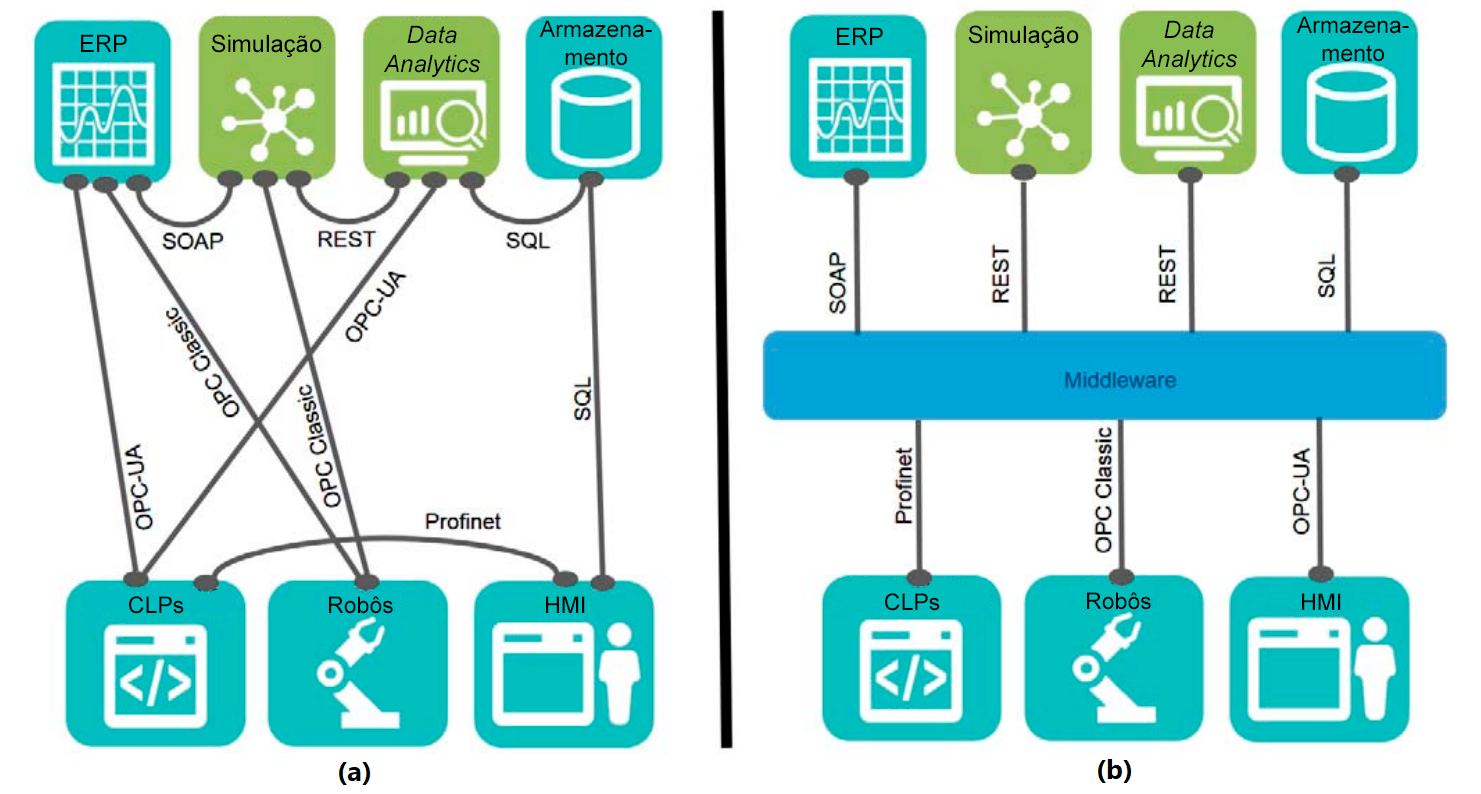
\includegraphics[width=0.9\textwidth]{middleware.png}
		\fonte{\citeonline{gosewehr2017middleware} (adaptado).}
	\end{figure}

	SOA está relacionada à ideia de uma Interface de Programação de Aplicação (\textit{Application Programming Interface} - API), que é o conjunto de rotinas e padrões estabelecidos por um \textit{software} para a utilização das suas funcionalidades por aplicativos externos.
	
	Para se disponibilizar um serviço por meio de uma API, o conceito de \textit{Web Services} (WS) é vastamente utilizado \cite{souit2013soa}. Os WSs podem ser vistos como um conceito padrão para facilitar a interoperabilidade, integração e reuso dos componentes de aplicações.
	
	\subsection{Web Services}

	Um \textit{Web Service} (WS) é uma interface que descreve uma série de operações acessíveis por meio de uma linguagem de descrição de serviços padronizada \cite{gottschalk2002webservices}. Um WS executa uma tarefa específica ou um conjunto de tarefas e retorna ao usuário o resultado da operação. Cada aplicação pode ter a sua própria linguagem, que é traduzida para uma linguagem comum, como um XML, JSON, CSV, etc.
	
	Por meio de WSs, as aplicações podem ser descritas, publicadas, localizadas e invocadas em uma rede de comunicação tipo WWW (\textit{World Wide Web}) \cite{souit2013soa}.
	
	A arquitetura de um WS é constituída por três atores básicos: o provedor de serviços, o repositório de serviços e o solicitante de serviços; e por três operações básicas: a publicação, a procura e a interação \cite{gottschalk2002webservices}. A \autoref{fig:webservice-componentes} ilustra os atores e a interação entre eles por meio das operações.
	
	\begin{figure}[htb]
		\centering
		\caption{Componentes de um WS e operações.}
		\label{fig:webservice-componentes}
		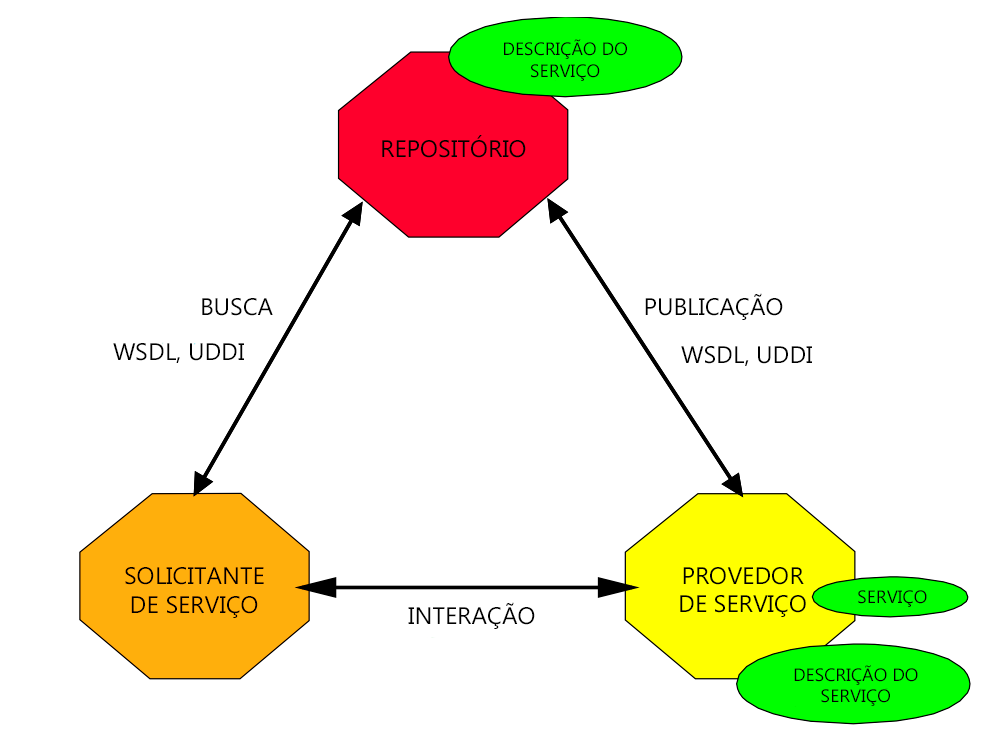
\includegraphics[width=0.8\textwidth]{webservice-componentes}
		\fonte{\citeonline{kreger2001webservices} (adaptado).}
	\end{figure}
	webservice-componentes
	Detalhadamente, os atores em um WS são:
	
	\begin{itemize}
		\item \textbf{Provedor de serviços}: Representa a plataforma que hospeda e fornece um determinado serviço, esta plataforma permite que clientes solicitem serviços e recebam suas respectivas respostas. O provedor de serviços é responsável também por fornecer uma descrição sobre o serviço prestado e publicar esta descrição em um repositório acessível pelo solicitante.
		
		\item \textbf{Repositório de serviços}: É uma plataforma acessível com a função de armazenar e fornecer a descrição sobre diversos WSs. Os WSs são descobertos pelo solicitante por meio do repositório para que assim possa decidir o serviço que melhor o atenda.
		
		\item \textbf{Solicitante de serviços}: É o ator que necessita de um determinado serviço e requisita a sua execução. O solicitante de serviço pode ser uma pessoa acessando um navegador ou uma aplicação realizando solicitações por meio de APIs.		
	\end{itemize}	
	
	Já as operações básicas em WS em detalhe são:
	
	\begin{itemize}
		\item \textbf{Publicação}: Publicação da descrição do serviço pelo provedor em um repositório para que o serviço se torne acessível ao público e os solicitantes possam localizá-lo.
		
		\item \textbf{Busca}: Busca e recebimento da descrição de um serviço. O solicitante pode receber a descrição do serviço pelo provedor ou por meio do repositório.
		
		\item \textbf{Interação}: Comunicação direta entre solicitante e provedor para o fornecimento de serviços. Nesta fase, o solicitante se decide por um determinado serviço dentre os disponíveis no repositório e inicia uma interação com o provedor por meio de uma API.
	\end{itemize}
	
	As etapas de interação entre as entidades são representadas por meio de diagrama UML na \autoref{fig:uml-webservice}. 
	
	\begin{figure}[htb]
		\centering
		\caption{Diagrama UML com os atores e interações em um WS.}
		\label{fig:uml-webservice}
		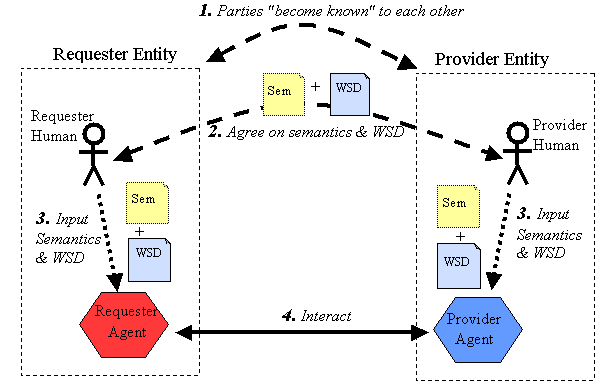
\includegraphics[width=1\textwidth]{uml-webservice}
		\fonte{\citeonline{booth2004webservice} (adaptado).}
	\end{figure}

	Neste diagrama a Semântica e a Descrição do Web Service (\textit{Web Service Description} -- WSD) representam os documentos com os quais ambas as partes devem concordar para que haja o efetivo fornecimento e consumo do serviço.
	
	O WSD define os formatos de mensagem, tipos de dados, protocolos de transporte e formatos de troca de dados que devem ser usados entre o solicitante e o provedor \cite{booth2004webservice}. O WSD representa um acordo que rege a mecânica de interação com esse serviço.
	
	Já a Semântica de um WS é o documento que compartilha o comportamento esperado de resposta deste serviço, pode ser explícito ou implícito, oral ou escrito, processável por máquina ou orientado a humanos, e pode ser um acordo legal ou um acordo informal \cite{booth2004webservice}.

	Os WSs se tornaram bastante atrativos, pois esse modelo pode ser aplicado com tecnologias acessíveis ao solicitante, em particular XML e HTTP, que podem ser acessadas pela maioria dos navegadores convencionais. A disponibilização de serviços interativos na \textit{Internet} se tornou muito popular e com isso surgem novos modelos de negócios como o SaaS (\textit{Software as a Service}), PaaS (\textit{Platform as a Service}), IaaS (\textit{Infrastructure as a Service}), etc.
	
	Dentro do mundo da Indústria 4.0 não é diferente. Ativos podem publicar suas funcionalidades em repositórios e executarem determinadas tarefas mediante solicitação por parte do solicitante, podendo assim serem classificados como uma manufatura como um serviço (\textit{Manufacturing as a Service}) \cite{annunziata2019maas, nichols2020maas, siepen2019maas}.
	
	\subsection{Transferência Representacional de Estado}
	
	A Transferência Representacional de Estado (\textit{Representational State Transfer} - REST) é uma arquitetura de \textit{software} que define padrões para acesso e disponibilização de \textit{Web Services} (WSs). Os WSs que seguem o padrão REST são denominados \textit{RESTful Services}.
	
	A arquitetura REST possibilita a interoperabilidade entre sistemas na \textit{Internet}, pois permite que os sistemas solicitantes acessem e manipulem representações textuais de recursos usando um conjunto uniforme e predefinido de operações sem estado \cite{ferris2004webservices}.
	
	Quando o HTTP é usado como protocolo de comunicação em um \textit{RESTful Service}, cada método do protocolo recebe um tipo de operação padrão do REST. A \autoref{tab:rest} mostra as possíveis operações e seus métodos HTTP correspondentes, quando este protocolo é utilizado.
	

	\begin{table}[htb]
		\centering
		\footnotesize
		\caption{Possíveis operações em um \textit{RESTful Service}.}
		\label{tab:rest}
		\begin{tabular}{p{2cm}p{2cm}p{8cm}}
			\hline
			\textbf{Operação} &
			\textbf{Método \newline HTTP} &
			\textbf{Resposta} \\[5mm]

			\hline
			Criação &
			POST &
			201 (Criado) \\[5mm]
			
			\hline
			Leitura &
			GET &
			200 (OK), 404 (Não encontrado)  \\[5mm]
			
			\hline
			Atualização &
			PATCH &
			200 (OK), 204 (Sem conteúdo), 404 (Não encontrado),405 (Não permitido) \\[5mm]
			
			
			\hline
			Exclusão &
			DELETE &
			200 (OK), 404 (Não encontrado), 405 (Não permitido) \\[5mm]
			
			\hline
		\end{tabular}
		\fonte{\cite{fielding2000architecture} (adaptado).}
	\end{table}

\section{Modelagem de sistemas}
\label{sec:modelagem}

	Sistemas são um conjunto de elementos interdependentes de modo a formar um todo organizado. Também pode ser entendido como um conjunto de órgãos funcionais, componentes, entidades, partes ou elementos e as relações entre eles, com um objetivo geral a ser atingido \cite{mulbert2005sistemas}.
	
	No contexto da Logística 4.0, um sistema pode ser definido como o conjunto de diferentes cadeias de suprimentos ligadas por meio de relacionamentos interorganizacionais, que fazem acontecer os fluxos envolvidos (de dinheiro, materiais, bens e informações) \cite{oliveira2016supplychain}.
	
	A modelagem e análise dos sistemas na cadeia de suprimentos é uma ferramenta para melhorar a eficiência da cadeia como um todo. As vantagens de sua utilização podem possibilitar a capacidade de capturar e entender o comportamento da rede, a reprodução e análise de diferentes cenários e soluções, previsibilidade de possíveis perturbações de mercado e melhoria nos processos de distribuição.
	
	Com a intensificação da globalização, é cada vez mais comum a criação de cadeias de suprimentos complexas, envolvendo várias organizações dispersas geograficamente. Por isso, as ferramentas de suporte à tomada de decisões podem auxiliar no sentido de fornecer uma solução mais adequada à dinâmica de diversas redes.
	A modelagem é uma das formas de auxílio à tomada de decisões e pode ser uma ferramenta útil para se entender as interações e melhorar a performance da CS \cite{oliveira2016supplychain}. 
	
	Um desafio para desenvolvimento de bons modelos nessa área é a adoção de metodologias claras que possam facilitar e agilizar o processo de se realizar a modelagem e a análise de aspectos da cadeia de suprimentos. Uma metodologia apresenta apenas um direcionamento sobre os procedimentos a serem tomados a fim de se atingir um objetivo, porém cada problema a ser analisado requer especificações diferentes, o que demanda adaptações dos procedimentos originais.
	
	\citeonline{miyagi1996controle} define os sistemas feitos pelo homem (\textit{man-made systems}) como sistemas de manufatura, transporte, comunicação, redes de computadores, etc. Estes sistemas seriam caracterizados por uma dinâmica decorrente da ocorrência de eventos e, portanto, são classificados como Sistemas a Eventos Discretos (SED).
	
	Um SED é uma classificação do sistemas de acordo com seu comportamento determinado pela ocorrência de eventos que alteram de forma discreta instantânea o estado do sistema \cite{miyagi1996controle}.
	
	Para a modelagem de SEDs, a aplicação de ferramentas como a Rede de Petri e suas variações como \textit{Production Flow Schema} (PFS) e \textit{Mark Flow Graph} (MFG) são formas de auxílio no desenvolvimento de sistemas de controle e automação.
	
	A utilização da técnica de PFS no contexto da I4.0 pode auxiliar no mapeamento das operações e interações entre os elementos do sistema, uma vez que a dinâmica de interação pode ser classificada com um SED. Neste trabalho o PFS é utilizado a fim de se indicar as operações e suas relações ao longo das camadas do RAMI4.0.
	
	\subsection{Production Flow Schema}
	
	O PFS (\textit{Production Flow Schema}) é uma técnica indicada para aplicação em diferentes níveis de modelagem, análise e controle de SEDs \cite{miyagi1996controle}.
	
	No PFS, os eventos são indicações de determinadas atividades, que por sua vez podem incluir vários outros eventos e estados organizados hierarquicamente.
	
	Por meio de modelos em PFS, é especificada a estrutura da arquitetura apresentada, indicando assim as interações de seus componentes. Além disso, com o PFS, os fluxos das operações podem ser descritos se forma desacoplada de qualquer tecnologia necessária para a implementação do sistema \cite{pisching2018equipmentrami}.
	
	Em um PFS deve haver a representação dos eventos discretos, portanto, qualquer processo produtivo representado em PFS apresentará os seguintes elementos estruturais:
	
	\begin{itemize}
		\item Atividades: Representação dos componentes ativos;
		\item Distribuidores: Representação dos componentes passivos;
		\item Arcos orientados: Representação das relações entre os componentes ativos  e passivos.
	\end{itemize}

	A \autoref{fig:pfs-elementos} descreve os elementos do PFS e sua representação gráfica.
	
	\begin{figure}[htb]
		\centering
		\caption{Elementos do PFS.}
		\label{fig:pfs-elementos}
		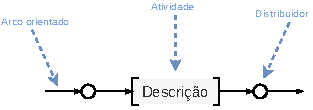
\includegraphics[width=1\textwidth]{pfs-elementos}
		\fonte{\citeonline{pisching2018pfs} (adaptado).}
	\end{figure}

	A atividade corresponde à realização de certas unidades ou conjuntos de operações, como um processamento, uma montagem, desmontagem, etc. Os distribuidores correspondem ao lugar de entrada e saída de itens ou a transição entre as diferentes atividades. Já os arcos orientados indicam a direção dos fluxos e a relação entre os eventos.
	
	Os arcos conectando a parte externa das atividades (horizontalmente) indicam um fluxo principal (primário), já os arcos conectando a parte interna da atividade (verticalmente) indicam um fluxo secundário \cite{miyagi1996controle}. 
	
	Um terceiro tipo de fluxo é usado para representar a integração entre interfaces das atividades e é indicado por meio de um arco conectando diretamente duas atividades. O arco indicador de interação de fluxo é usado para modelar interações entre diferentes níveis, como operações de solicitação e resposta \cite{pisching2018pfs}.
	
	Os tipos de fluxo na representação em PFS é mostrada na \autoref{fig:pfs-fluxos}.
	
	\begin{figure}[htb]
		\centering
		\caption{Tipos de fluxo no PFS.}
		\label{fig:pfs-fluxos}
		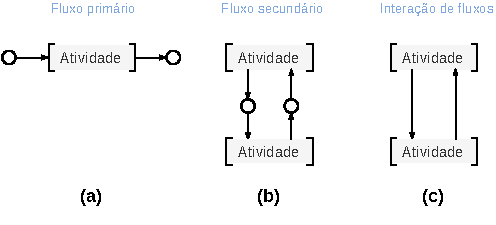
\includegraphics[width=1\textwidth]{pfs-fluxos}
		\fonte{\citeonline{pisching2018pfs} (adaptado).}
	\end{figure}
	
	Os fluxos de processo do sistema em PFS são modelados por meio de uma abordagem \textit{top-down}, assim os resultados podem ser refinados sucessivamente detalhando-se a cada iteração a atividade representada. A modelagem do sistema em PFS, portanto, parte de um alto nível de abstração, seguido de sucessivos refinamentos detalhando o modelo a cada nível.
	
	Desta forma, o PFS representa uma linguagem de alto nível independente de tecnologias e fabricantes para modelar os processos do sistema. A relevância de se adotar uma linguagem natural para a representação do sistema como o PFS está na padronização da comunicação com especialistas de diferentes áreas, como arquitetos, engenheiros e \textit{designers}. Assim, há uma efetiva comunicação sobre a interação entre as partes de um sistema e sobre os fluxo de elementos e operações em diferentes níveis do sistema em análise, como, por exemplo, produtos, ordens de serviço, máquinas, informações de sensores, etc.

	
	
	
	